\documentclass[12pt,a4paper]{article}

\usepackage[utf8]{inputenc}
\usepackage{amsmath}
\usepackage{graphicx}
\usepackage{float}
\usepackage{listings}

\begin{document}

\title{MI-PAA 2015 5.ukol \\
Řešení problému vážené splnitelnosti booleovské formule pokročilou iterativní metodou
}
\author{Tomas Nesrovnal\\nesrotom@fit.cvut.cz}
\date{\today}
\maketitle

\newpage

% https://edux.fit.cvut.cz/courses/MI-PAA/homeworks/05/start

\section{Uvod do problemu}

\subsection{Definice}
Je dána booleovská formule $F$ proměnnných $X=(x1, x2, … , xn)$ v konjunktivní normální formě (tj. součin součtů). Dále jsou dány celočíselné kladné váhy $W=(w1, w2, … , wn)$. Najděte ohodnocení $Y=(y1, y2, … , yn)$ proměnných $x1, x2, … , xn$ tak, aby $F(Y)=1$ a součet vah proměnných, které jsou ohodnoceny jedničkou, byl maximální.

Je přípustné se omezit na formule, v nichž má každá klauzule právě 3 literály (problém 3 SAT). Takto omezený problém je stejně těžký, ale možná se lépe programuje a lépe se posuzuje obtížnost instance (viz Selmanova prezentace v odkazech).

\subsection{Priklad}
$x1'$ značí negaci $x1$.

$n = 4$

$F = (x1 + x3' + x4).(x1' + x2 + x3').(x3 + x4).(x1 + x2 + x3' + x4').(x2' + x3).(x3' + x4')$ 

$W = (2, 4, 1, 6)$


Přípustné konfigurace, kde $F=1$ (řešení):

$X = \{x1, …,xn\} = \{0, 0, 0, 1\}, S = 6$

$X = \{x1, …,xn\} = \{1, 0, 0, 1\}, S = 2 + 6 = 8 $ (optimální)

$X = \{x1, …,xn\} = \{1, 1, 1, 0\}, S = 2 + 4 + 1 = 7$

\subsection{DIMACS CNF format}

Instance z prikladu zapsana v DIMACS CNF formátu vypada nasledovne:

\begin{verbatim}
c Priklad CNF
c 4 promenne a 6 klauzuli
c kazda klauzule konci nulou (ne novym radkem)
p cnf 4 6
1 -3 4 0
-1 2 -3 0
3 4 0
1 2 -3 -4 0
-2 3 0
-3 -4 0
\end{verbatim}

Tento format neobsahuje vahy. Symbol c znamena komentar. Radek zacinajici p ve formatu "p cnf nbvar nbclauses" rika, ze instance je v CFN formatu, ma nbvar promennych a obsahuje nbclauses klauzoli. Pridame proto radek zacinajici w za kterem budou nasledovat vahy. Ukazova instance z predhoziho prikladu ma tedy tento format:

\begin{verbatim}
c Priklad CNF
c 4 promenne a 6 klauzuli
c kazda klauzule konci nulou (ne novym radkem)
p cnf 4 6
w 2 4 1 6
1 -3 4 0
-1 2 -3 0
3 4 0
1 2 -3 -4 0
-2 3 0
-3 -4 0
\end{verbatim}

\subsection{3SAT}

Protoze je 3SAT stejne tezky, budeme pracovat pouze s nim. Lepe se bude posuzovat obtiznost instanci a take se snadneji vytvareji, hledaji testovaci data.


\section{Algoritmus a implementace}

\subsection{Simulovana evoluce}
Nejprve jsem implementoval zakladni simulovanou evoluci. Pouzita byla jen mutace, dvoubodove krizeni a turnajova selekce. Protoze algoritmus nedosahoval dobrych vysledku a protoze jsem simulovanou evoluci resil predchozi ulohu batohu, rozhodl jsem se od tohoto reseni upustit a zkusit simulovane zihani.

\subsection{Simulovane zihani}
Algoritmus simulovaneho zihani vychazi z algoritmu Hill climbing.

\subsubsection{Hill climbing}
Hill climbing vyuziva dosud nejlepsiho nalezeneho reseni. Analogicky k splhani do kopce se rozhlizime (generujeme dalsi body z nalezeneho reseni) a jdeme nahoru (tedy pokud je vygenerovany bod vys, jdeme na nej). Generovanim dalsich bodu se v nasem pripade mysli prohozeni hodnoty nektere promenne.

Nejvetsim problemem Hill climbingu je uvaznuti v lokalnich extremech. Resenim by bylo s nejakou pravdepodobnosti prijmout i horsi reseni. Na tomto principu funguje simulovane zihani.

\subsubsection{Simulovane zihani}
Anglicky Simulated annealing, jinak cesky Simulovane propousteni nebo i simulovane ochlazovani.

Je to tedy algoritmus podobny Hill climbingu, ktery ale s urcitou a postupne klesajici pravdepodobnosti prijima horsi stavy, cimz je schopen vyvaznout z lokalnich extremu.

Algoritmus zacne s nejakou pocatecni telplotou a po ekvilibrium krocich ji snizi vynasobenim ochlazovanim faktorem. V kazdem kroku pak vygeneruje novy stav. Pokud je jeho cena lepsi, prijme se jako soucasne nejlepsi nalezene reseni. Pokud ne, je jeste $e^{-d/t}$ (kde d je rozdil cen mezi soucasnym nejlepsim resenim a nove vygenerovanym a t je soucasna teplota) sance, ze se take stav prijme. To nam umozni vyvaznuti z lokalnich extremu.

\begin{itemize}
\item ti je pocateni teplota
\item te je konecna teplota ($te < ti$)
\item eq je hodnota equlibria ($0 < eq$)
\item cf je ochlazovaci faktor ($0 < cf < 1$)
\end{itemize}

Zde je zjednoduseny zdrojovy kod v jazyce C:

\begin{lstlisting}[frame=single]
for (double t = ti; te < t; t *= cf) {
  for (int i = 0; i < eq; i++) {
    state_next = state_genenerate_next(state);
    double d = cost(state) - cost(state_next);
    if (d < 0 || randd() < pow(M_E, -d / t)) {
      state_swap(&state, &state_next);
      continue;
    }
  }
}
\end{lstlisting}

\section{Reseni}
Je nekolik velmi dulezitych veci nad kterymi je potreba se zamyslet pro dobrou implementaci algoritmu. Za prve je to spravne nastaveni parametru pro simulovane zihani - tedy pocatecni a koncove teploty, chladici faktor a hodnota ekvilibria. Za druhe je to pocatecni reseni. Dale je to vhodne zvolena cenova funkce, ktera ohodnoti stav cislem.


\subsection{Cenova funkce}

Stavy jsou reprezentovany binarnim vektorem, ktery znaci ohodnoceni literalu. Stav muze byt bud validni, nebo nevalidni. Pokud se $S$ ohodnoceni formule $F$ a $F(S) = 0$, znamena to, ze formule neni splnena, coz je podle zadani nevadlidni reseni. Naopak pokud $F(S) = 1$, je formule splena a stav je tedy validni.

Cilem je najit takove validni reseni, ktere ma nejvetsi soucet vah. Validni reseni s velkou vahou by tedy mely mit velkou cenu. Je ale potreba zohlednit to, ze nejaky stav muze byt nevalidni, ale je blizko nejakeho validniho reseni s velkou cenou.

\subsubsection{Promenne v cenovych funkcich}

Nasleduje vycet cenovych funkci. Malym c budu oznacnovat pocet splnenych klausoli a velkym C celkovy pocet klausoli. Velkym W oznacim sumu vsech vah: $W = \sum_{i=1}^{n}{w_i}$. Malym w oznacim sumu vah pro splnene klauzole $w = \sum_{i=1}^{n}{y_i w_i}$

\subsubsection{Cenova funkce $cost1$}

$$ cost1(Y) = F(Y)W + \frac{c}{C}w $$


\subsubsection{Cenova funkce $cost1$}

$$
 cost2(Y) =
  \begin{cases}
    W + w       & \quad \text{if } F(Y) = 1 \\
    \frac{c}{C}W  & \quad \text{if } F(Y) = 0 \\
  \end{cases}
$$


\subsection{Nastaveni parametru}
Nastaveni parametru je tezky ukol, exi

\subsection{Kriterium ukonceni}

Vypocet skonci po tom, co se teplota snizi na predem stanovenou mez. Je tedy mozne, ze zadne validni reseni nebude nalezeno, prestoze jich v instanci existuje hodne. Je to hlavne z toho duvodu, ze na beh algoritmu ma z velke casti nahoda.


\subsection{Opakovani vypoctu}

Protoze je algoritmus nahodny na nahode, budeme vypocet opakovat 100 krat a vysledkem bude prumerna hodnota.


\subsection{Pocatecni stav}
Existuje nekolik moznosti jak zvolit pocatecni stav.

Prvni moznosti je zacit se stavem, ktery vsechny literaly odhonoti bud 0, nebo 1. Vzhledem k povaze vstupnich dat, ktere muzou byt jakekoliv bysme ale pro nejake instance mohli touto taktikou vypocet velice znekvalitnit. Lepsim resenim bude priradit kazdemu literalu nahodne bud 0 nebo 1.

Druhou moznosti je pokusit se vygenerovat nejaky validni stav, nebo pouzit sat resic a vychazet z neho. Timto zpusobem bysme pravdepodobne zacinali v lokalnim extremu, kterym se ale chceme vyvarovat.

Pocatecni stav bude tedy vygenerovan zcela nahodne.

\subsection{Generovani nasledniku}
Generovani naslednika znamena vzit nejaky stav a nejakou modifikaci vytvorit novy stav, velice blizky tomu prvnimu.

Nejjednodussi metodou je negace soucasne hodnoty nahodneho literalu.

Dalsi moznosti je ta, ktera se snazi vygenerovat validni nasledniky. Vezme nahodnou nesplnenou klauzoli a zneguje nejaky nahodny literal tak, aby klauzole byla validni.


\subsection{Optimalizace algoritmu}

Po sepsani textu vyse mi doslo, ze algorimus se da naprogramovat optimalneji. 

\subsubsection{Generovani jedinecnych nasledniku}

Naslednici se generuji nahodne, je tedy mozne, ze se za jedno ekvilibrium (tedy za stejne teploty) vyzkousi stejny naslednik nekolikrat. To nicemu nevadi, pokazde se vygeneruje sance, s jakou se pripadne horsi reseni prijme. Prakticky mi to prijde ale velice neprakticke, proto po zmene teploty nahodne vygeneruji indexy bitu, ktere se budou menit. Tim se take vytvori horni mez pro hodnotu ekvilibira a to pocet promennych. Vetsi pocet iteraci v ekvilibriu nema cenu, protoze bysme zkouseli stejne stavy vicekrat.

\subsubsection{Kopirovani stavu}

Ciste technickou zalezitosti je pak kopirovani stavu pri generovani jeho naslednika. Prestoze je funkce memcpy v C rychla a optimalizovana, muzeme se ji vyhnout tim, ze pri generovani naslednika budeme rovnou upravovat nejlepsi stav a v pripade, ze naslednika neprijmeme, vratime nejlepsi reseni do puvodniho stavu.

\subsubsection{Dalsi mozne optimalizace}

Dalsi optimalizaci by mohlo byt drzeni si uplne nejlepsiho nalezeneho stavu. Nebo nepocitani ceny soucasneho stavu, pokud se nezmenil. To jsem ale neimplementoval.


\subsubsection{Optimalizovany algoritmus}

Zjednoduseny zdrojovy kod v jazyce C:

\begin{lstlisting}[frame=single]
for (double t = ti; te < t; t *= cf) {
  p = generate_random_permutation();
  for (int i = 0; i < eq; i++) {
    double cost_state = cost(state);
    state[p[i]] = swap_bit(state[p[i]]);
    double d = cost_state - cost(state);
    if (d < 0 || randd() < pow(M_E, -d / t)) {
      continue;
    }
    state[p[i]] = swap_bit(state[p[i]]);
  }
}
\end{lstlisting}



\section{Instance}

\subsection{Generator G2}

Pro generovani zkusebnich dat jsem si nejprve stahnul generator G2, ktery byl na studentskem webu fit-wiki. Generator pracuje na tom principu, ze nahodne vygeneruje nejake reseni a pak podle nej dopocita klauzole, literaly i vahy. Upravene zdrojove kody tohoto generatoru jsou soucasti zdrojovych kodu. Po par experimentech bylo ale jasne, ze generator nezarucuje, ze nalezene reseni je globalni optimium. Proto jsem si naprogramoval brute force resic, ktery mi vzdy zarucene globalni optimum najde. 

\subsection{SATLIB}

SATLIB knihovna obsahuje take instance 3SAT. Testovaci data maji navic pomer poctu klauzoli a poctu literalum blizici se cislu 4.3. Podle clanku Stochastic Search And Phase Transitions:AI Meets Physics od Barta Selmana jsou to tedy ty nejtezsi instance problemu.

Pro kazdy literal byla nahodne pomoci bashoveho skriptu vygenerovana vaha v rozsahu 20 az 60.

\section{Experimentalni reseni}

\subsection{Postup mereni}
Mereno bylo na notebooku s Intel(R) Core(TM) i3-2328M Processor (3M Cache, 2.20 GHz), 8GB RAM, gcc 4.9.2 (-Ofast), OS GNU/Linux Lubuntu 14.04.3 64bit.

Mereny byly instance 3SAT problemu z knihovny SATBLIB.

\subsection{Volba parametru}

\subsubsection{Koncova teplota}
Koncovou teplotu jsem empiricky zvolil na $te = 0.01$. Je to podle me dostatecne male cislo na to, aby se ke konci vypoctu prijmulo horsi reseni.

\subsubsection{Pocatecni teplota}
U pocatecni teploty jsem nezvolil zadne pevne cislo. Zalezi totiz na velikosti vah. Proto jsem empiricky zvolil tento vzorec na vypocet pocatecni teploty:

$$ ti = PocetLiteralu * MaximalniVaha * 10 $$



\subsection{Vyber cenove funkce}






%\begin{figure}[H]
%	\caption{Vliv velikosti tournamentu}
% 	\centerline{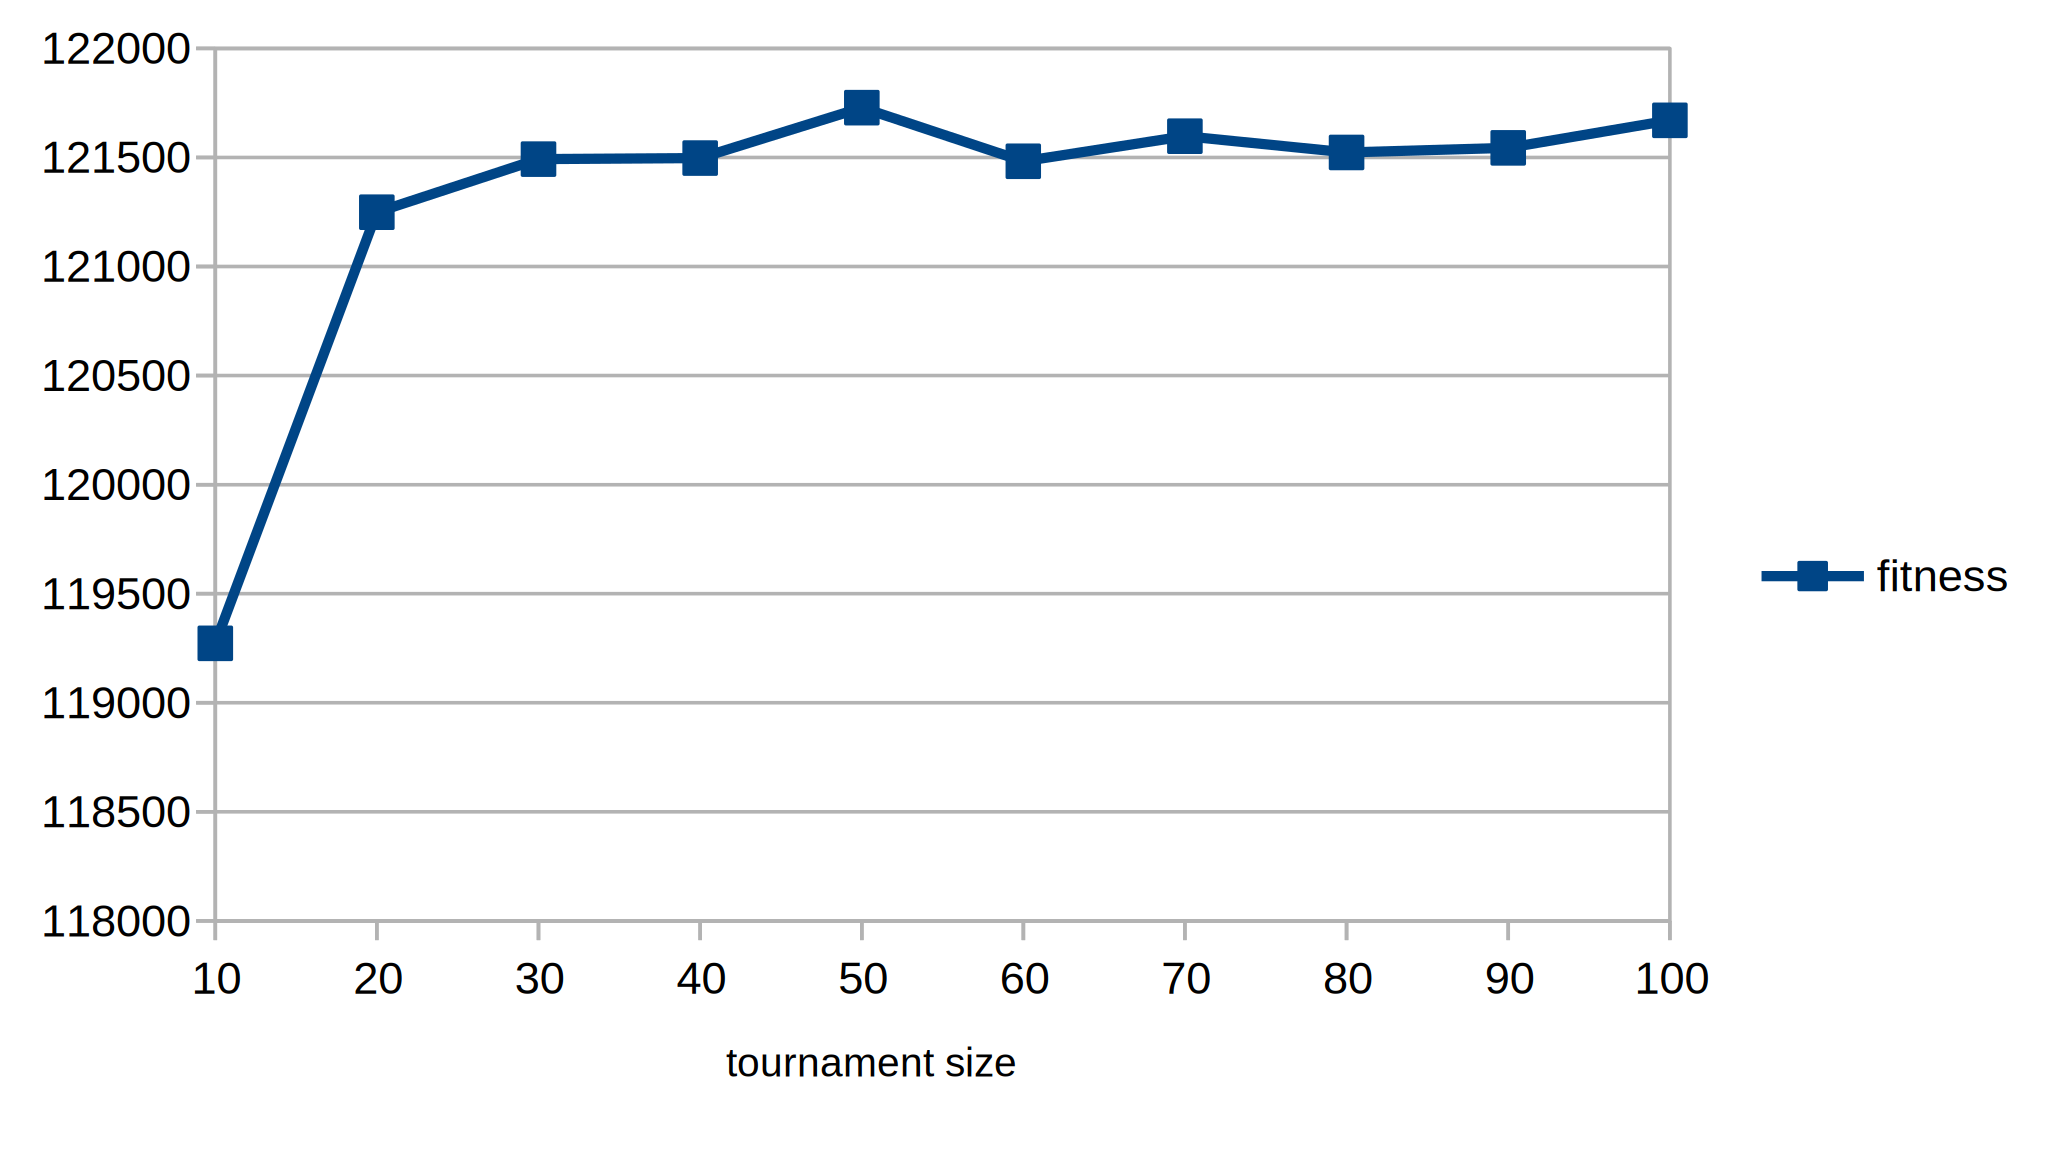
\includegraphics{tournament.pdf}}
%\end{figure}


%%%%%%%%%%%%%%%%%%%%%%%%%%%%%%%%%%%%%%%%%%%%%%%%%%%%%%%%%%%%%%%%%%%%%%%%%%%%%%
\end{document}
